\documentclass[presentation]{beamer}
\usepackage{common}
\usepackage{arydshln}

\newcommand{\cscat}[1]{$\langle\text{{\itshape#1}}\rangle$}
\newcommand{\csopt}[1]{{\itshape[}#1{\itshape]}}
\newcommand{\csalt}[1]{{\itshape(#1)}}
\newcommand{\op}[1]{\alert{`\texttt{#1}'}}
\newcommand{\operand}[1][\ldots]{{\normalcolor#1}}
\newcommand{\literal}[1]{\texttt{\alert{#1}}}
\newcommand{\bs}{$\backslash$}
\newcommand{\codepath}[1]{../../code/lecture-06/#1}

\newcommand{\kva}[2]{\alert{\lbrack}\cscat{#1}\alert{\rbrack=}\cscat{#2}}
\newcommand{\kvb}[2]{\alert{\{}\cscat{#1}\alert{,}\cscat{#2}\alert{\}}}

\AtBeginSubsection[]
{
  \begin{frame}<beamer>
    \frametitle{Next In Line\ldots}
    \tableofcontents[currentsection,currentsubsection]
  \end{frame}
}

\title[\lecturecode{06b}]{06b \\ \dotnet Collections}

\author[Giovanni Ciatto]{Giovanni Ciatto\\\texttt{giovanni.ciatto@unibo.it}}

\begin{document}

\frame[label=coverpage]{\titlepage}

\section{Collections in General}

\begin{frame}{Overview}
  \begin{itemize}

    \item Collections are data structures aimed at containing data
    %
    \begin{itemize}
      \item they enable and ease the design an implementation of algorithms and types
    \end{itemize}

    \vfill

    \item Most developers only rarely build their own collections
    
    \vfill

    \item More commonly they rely on pre-existing collections
    %
    \begin{itemize}
      \item provided by either standard libraries or thid-party libraries
      \item possibly, barely exploiting or combining them
    \end{itemize}

    \vfill

    \item Therefore, learning \alert{how to use} common collections is far more useful than learning how they internally work
    
    \vfill

    \item We here provide a brief summary of \alert{which sorts} of collections you may find in \alert{virtually all} programming languages
    %
    \begin{itemize}
      \item \ldots and what you can expect from each one
    \end{itemize}    
    
  \end{itemize}
\end{frame}

\begin{frame}[allowframebreaks]{Main sorts of Data Structures}

  \begin{block}{Collection / Bag}
    \begin{center}\itshape
      General sort of data structure containing an \alert{arbitrary} amount of \alert{items}
    \end{center}
    %
    \begin{itemize}
      \item commonly, items are all of the same \alert{type}
      \item no assumption on the \alert{ordering} or \alert{duplication} of items
      \item may generally support counting, enumerating, adding, removing and checking the presence of items
    \end{itemize}
  \end{block}

  \begin{exampleblock}{Sorts of operations}
    \begin{description}
      \item[counting] $\rightarrow$ computing \alert{how many} items the collection contains
      \item[emerating] $\rightarrow$ \alert{stepping through all} items the collection
      \item[adding] $\rightarrow$ \alert{inserting one} more item into the collection
      \item[removing] $\rightarrow$ \alert{taking out a particular} item from the collection 
      \item[checking presence] $\rightarrow$ computing \alert{if} an item is \alert{contained} in the collection 
      \item[getting/reading] $\rightarrow$ \alert{selecting a particular} item in the collecton (without altering it) 
      \item[accessing] $\rightarrow$ either reading or removing
    \end{description}
    %
    \begin{itemize}
      \item Some operation may be \alert{lacking} or \alert{constrained}
      %
      \begin{itemize}
        \item depending on the nature of the collection
      \end{itemize}

      \item \alert{Bulk} operations may be constructed on top of \alert{elementary} ones
      %
      \begin{itemize}
        \item[eg] adding/removing/getting several items at once
      \end{itemize}
    \end{itemize}
  \end{exampleblock}

  \begin{block}{\textbf{List}, i.e. a particular sort of \textbf{collection}\ldots}
    \begin{center}\itshape
      \ldots storing an \alert{unlimited} amount of items in an \alert{orderly} fashion, possibly \alert{with repetition}
    \end{center}
    %
    \begin{itemize}
      \item items can be accessed via their \alert{index}, i.e. their position in the list
      \item items can be added at the \alert{beginning}, or the \alert{ending} of the list, as well as at a \alert{given index}
      \item enumeration is coherent with indexing
    \end{itemize}
  \end{block}

  \begin{block}{\textbf{Array}, i.e. a particular sort of \textbf{list}\ldots}
    \begin{center}\itshape
      \ldots storing a \alert{fixed} amount of items
    \end{center}
    %
    \begin{itemize}
      \item arrays are usually \alert{contigously allocated} in memory
      \item ideal for low-level programming
    \end{itemize}
  \end{block}

  \begin{block}{\textbf{Queue}, i.e. a particular sort of \textbf{list}\ldots}
    \begin{center}\itshape
      \ldots only supporting \alert{first-in-first-out (FIFO)} access/add mode for its items
    \end{center}
    %
    \begin{itemize}
      \item only the \alert{first item} (a.k.a. \alert{head}) in the queue can be accessed
      \item items can only be \alert{appended}, i.e. added at the end of the queue (a.k.a. \alert{tail})
    \end{itemize}
  \end{block}

  \begin{block}{\textbf{Stack}, i.e. a particular sort of \textbf{list}\ldots}
    \begin{center}\itshape
      \ldots only supporting \alert{last-in-first-out (LIFO)} access/add mode for its items
    \end{center}
    %
    \begin{itemize}
      \item only the \alert{last item} (a.k.a. \alert{top}) in the stack can be accessed
      \item items can only be \alert{appended}, i.e. added at the end of the stack
    \end{itemize}
  \end{block}

  \begin{block}{\textbf{Deque} (double-ended queue), i.e. a particular sort of \textbf{list}\ldots}
    \begin{center}\itshape
      \ldots only supporting \alert{FIFO and LIFO} access/add modes for its items
    \end{center}
    %
    \begin{itemize}
      \item only the \alert{last or the first item} in the list can be accessed
      \item items can only be added at the \alert{beginning or the ending} of the list
    \end{itemize}
  \end{block}

  \begin{block}{\textbf{Set}, i.e. a particular sort of \textbf{collection}\ldots}
    \begin{center}\itshape
      \ldots storing an \alert{unlimited} amount of \alert{different} items of the \alert{same type}, \alert{regardless of their order}
    \end{center}
    %
    \begin{itemize}
      \item duplicates are \alert{not} allowed
      \item no assumption on the enumeration ordering
    \end{itemize}
  \end{block}

  \begin{block}{\textbf{Multiset}, i.e. a particular sort of \textbf{collection}\ldots}
    \begin{center}\itshape
      \ldots storing an \alert{unlimited} amount of items of the \alert{same type}, \alert{regardless of their order}
    \end{center}
    %
    \begin{itemize}
      \item keeps track of \alert{how many} duplicates exist for each item
      \item no assumption on the enumeration ordering
    \end{itemize}
  \end{block}

  \begin{block}{\textbf{Dictionary} / \textbf{Map}, i.e. a particular sort of \textbf{collection}\ldots}
    \begin{center}\itshape
      \ldots storing an \alert{unlimited} amount of items of the \alert{same type}, \alert{indexed by keys} of some \alert{other type}
    \end{center}
    %
    \begin{itemize}
      \item represents a function from the \alert{set of admissible keys} to the \alert{set of admissible values}
      \item each admissible key may correspond to \alert{at most 1} admissible value
      \item the same value may correspond to several keys
      \item items are added/accessed by specifying their key
      \item removing keys means removing items
      \item adding an item to a pre-existing key means replacing the item
    \end{itemize}
  \end{block}

  \begin{exampleblock}{\textbf{Multi-dimensional} arrays\ldots}
    \begin{center}\itshape
      \ldots can be conceived as \alert{dictionaries} of \alert{fixed size}
    \end{center}
    %
    \begin{itemize}
      \item where the set of admissible keys consists of \alert{vectors of integers}
      \item where keys cannot be removed or added
    \end{itemize}
  \end{exampleblock}

  \begin{exampleblock}{\textbf{Lists}\ldots}
    \begin{center}\itshape
      \ldots can be conceived as \alert{dictionaries} whose keys are \alert{non-negative integers}
    \end{center}
  \end{exampleblock}

  \begin{block}{\textbf{Tuple}, i.e. a particular sort of \textbf{list}\ldots}
    \begin{center}\itshape
      \ldots storing an \alert{fixed} amount of items of the \alert{same type}, of \alert{different types}
    \end{center}
    %
    \begin{itemize}
      \item items in the \alert{same position} \emph{must} be of the \alert{same type}
      \item items in \alert{different positions} \emph{may} be of \alert{different types}
    \end{itemize}
  \end{block}

\end{frame}

\begin{frame}[allowframebreaks]{Operation Modes for Collections}
  \begin{block}{\textbf{Mutable} collections}
    \begin{center}\itshape
     The \alert{pool of items} of a collection \alert{may change}, via the operation it supports
    \end{center}
    %
    \begin{itemize}
      \item effect of \alert{adding} an item $\rightarrow$ the collection contains \alert{one more item} than before
      \item effect of \alert{removing} an item $\rightarrow$ the collection contains \alert{one lesss item} than before
    \end{itemize}
  \end{block}

  \begin{block}{\textbf{Immutable} collections}
    \begin{center}\itshape
     The \alert{pool of items} of a collection \alert{never changes}
    \end{center}
    %
    \begin{itemize}
      \item only \alert{reading items} and \alert{creating novel instances} of the collection is supported
      \item to \alert{add} an item $\rightarrow$ a \alert{copy} of the collection is \alert{created}, containing \alert{one more} item
      \item to \alert{remove} an item $\rightarrow$ a \alert{copy} of the collection is \alert{created}, containing \alert{one less} item
    \end{itemize}
  \end{block}

  \begin{alertblock}{Mutable vs. Immutable}
    \begin{itemize}
      \item Mutable collections are commonly \alert{edit-efficient}
      %
      \begin{itemize}
        \item they are often \alert{error-prone}, as they may be subject to \alert{side-effects}
        \item furthermore, they complicate the design/implementation of \alert{concurrent} programs
      \end{itemize}

      \item Immutable collections are commonly \alert{read-efficient}
      %
      \begin{itemize}
        \item they simpler to design and use, and simplify the design of programs
        \item they can be used ``as-is'' in \alert{concurrent} programs
        \item they are slower when several edits must be performed to the same pool of data
      \end{itemize}
    \end{itemize}
  \end{alertblock}

  \begin{exampleblock}{Remarks}
    \begin{itemize}
      \item Mutable collections can be used \alert{immutably}, upon need
      %
      \begin{itemize}
        \item just by avoiding to modify them!
      \end{itemize}

      \item Our suggestion:
      %
      \begin{center}\itshape\small
        prefer an immutable design/usage, switch to mutable when strictly needed
      \end{center}
    \end{itemize}
  \end{exampleblock}
\end{frame}

\section{Collections in \dotnet}

\subsection{Overview}

\begin{frame}[allowframebreaks]{\dotnet{} Collections Overview}

  \begin{itemize}
    \item \dotnet comes with a number of built-in collection-related interfaces and classes
    \item They are organised in several namespaces and adhere to an articulated type hierarchy
    \item They can be freely exploitable in any custom \dotnet program/library
  \end{itemize}

  \begin{block}{Namespaces}\small
    \begin{description}
      \item[\texttt{System.Collections}] $\rightarrow$ all collection-related types
      \item[\texttt{System.Collections.Generic}] $\rightarrow$ all collection-related \alert{generic} types 
      \item[\texttt{System.Collections.Immutable}] $\rightarrow$ \alert{immutable \& generic} collection types
      \item[\texttt{System.Collections.Specialized}] $\rightarrow$ some type-specific implementation of collections 
    \end{description}
  \end{block}
\end{frame}

\begin{frame}[allowframebreaks]{Generic Collections and their Type Hierarchy}
  \begin{center}
    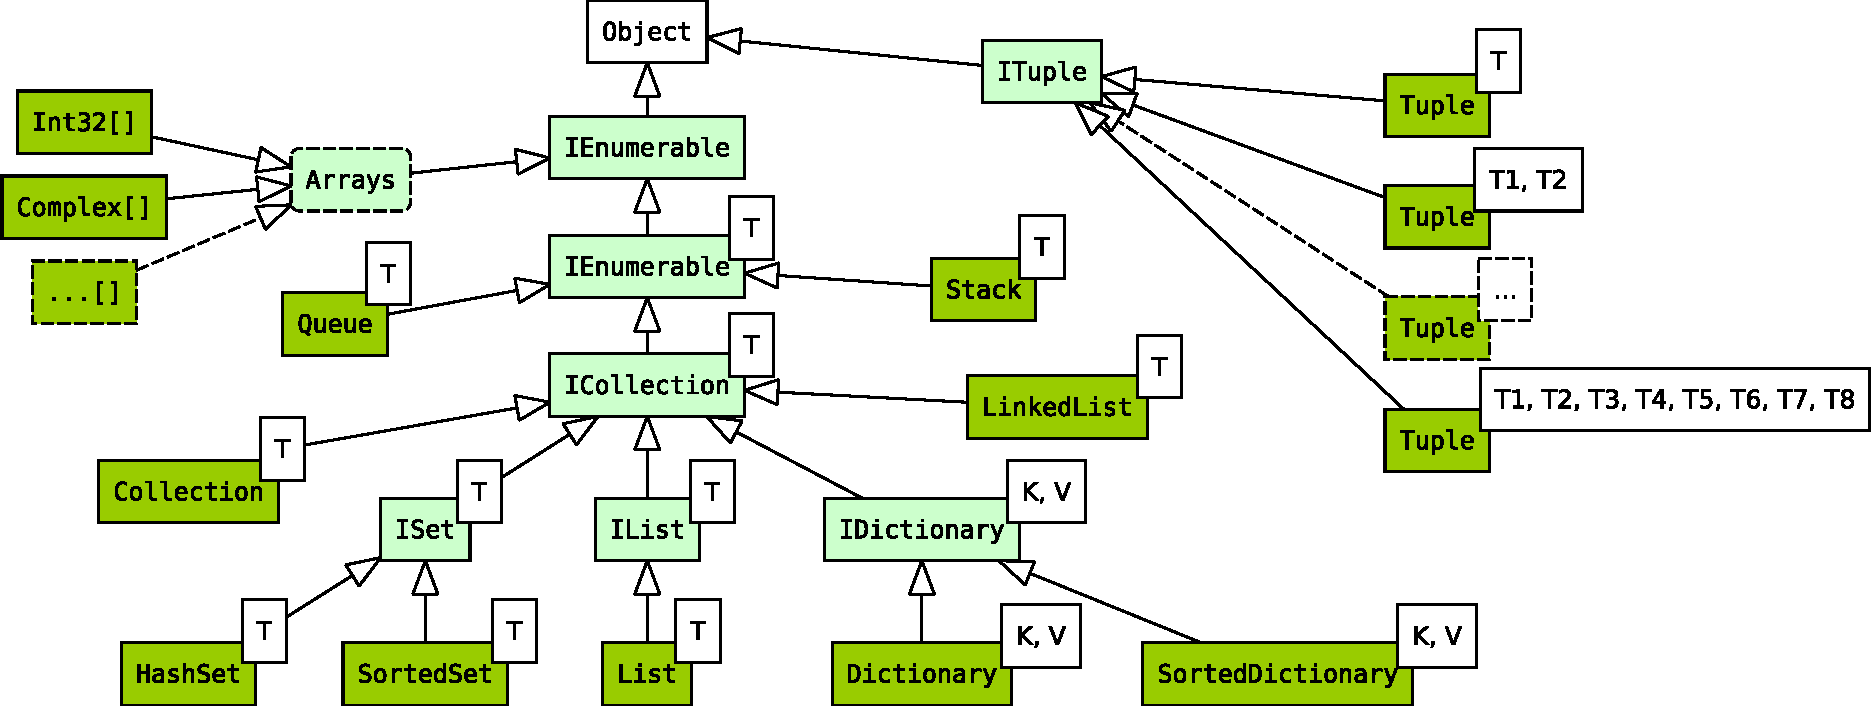
\includegraphics[width=\linewidth]{img/dotnet-collections.pdf}
  \end{center}
  %
  \begin{itemize}
    \item Notice the many \alert{type parameters} (while rectangles)
    \item All dark-green boxes represent classes which can be exploited in everyday programming
  \end{itemize}

  \begin{block}{\texttt{IEnumerable} is the type of all data structures\ldots}
    \begin{center}\itshape
      \ldots containing a number of \alert{\texttt{object}s}, which can be \alert{enumerated}
    \end{center}
  \end{block}

  \begin{block}{\texttt{IEnumerable<T>} is the type of all \texttt{IEnumerable}s\ldots}
    \begin{center}\itshape
      \ldots containing a number of instances of \alert{\texttt{T}}, which can be \alert{enumerated}
    \end{center}
  \end{block}

  \begin{block}{\texttt{ICollection<T>} is the super-type of all collections}
    Most notably, it is the super-type of:
    %
    \begin{description}
      \item[\texttt{ISet<T>}] i.e. the type of all \alert{sets} whose items are of type \alert{\texttt{T}}
      \item[\texttt{IList<T>}] i.e. the type of all \alert{lists} whose items are of type \alert{\texttt{T}} 
      \item[\texttt{IDictionary<K, V>}] i.e. the type of all \alert{maps} whose \alert{keys} (resp. \alert{values}) are of type \alert{\texttt{K}} (resp. \alert{\texttt{V}})
      %
      \begin{itemize}
        \item in this case \texttt{T} $\equiv$ \texttt{\alert{KeyValuePair<K, V>}}
        \item[ie] a structure defined in \texttt{System.Collections.Generic}
      \end{itemize} 
    \end{description}
  \end{block}

  \begin{block}{\texttt{ITuple} is the super-type of all sorts of tuples}
    Most notably, it is the super-type of:
    %
    \begin{description}
      \item[\texttt{Tuple<T1, T2>}] i.e. the type of all \alert{pairs} whose \alert{first} item is of type \alert{\texttt{T1}} and whose \alert{second} item is of type \alert{\texttt{T2}}
      \item[\texttt{Tuple<T1, T2, T3>}] i.e. the type of all \alert{triples} whose \alert{first} item is of type \alert{\texttt{T1}}, whose \alert{second} item is of type \alert{\texttt{T2}}, whose \alert{third} item is of type \alert{\texttt{T3}}
      \item[\vdots]
    \end{description}
  \end{block}

  \begin{exampleblock}{Remarks}
    \begin{itemize}
      \item Most of these types are in \texttt{System.Collections.Generic}
      \item All \alert{sorts} of \alert{arrays} and collections are \alert{enumerable}
      \item Tuples are \alert{not} enumerable
      \item Surprisingly, \texttt{Queue}s, \texttt{Stack}s, and \texttt{LinkedList}s are \alert{not} \texttt{IList}s
      \item Another hierachy exists, rooted in \texttt{ICollection}, for \alert{non-generic} types
      %
      \begin{itemize}
        \item these are contained into \texttt{System.Collections}
      \end{itemize}

      \item Another hierachy exists, rooted in \texttt{IReadOnlyCollection<out T>}, for \alert{read-only} types
      %
      \begin{itemize}
        \item these are contained into \texttt{System.Collections.Generic}
      \end{itemize}

      \item Other types exist, named \texttt{IImmutable*<T>}, for \alert{immutables} types
      %
      \begin{itemize}
        \item these are contained into \texttt{System.Collections.Immutable}
      \end{itemize}
    \end{itemize}
  \end{exampleblock}
\end{frame}

\subsection{Enumerables}

\begin{frame}[allowframebreaks]{The \texttt{foreach} construct}
  \begin{block}{For-Each Construct}

    \begin{center}\ttfamily
        foreach (\cscat{Type} \cscat{Variable} in \cscat{Container}) \{ \cscat{Block} \}
    \end{center}
    %
    \begin{itemize}
        \item where \texttt{\cscat{Variable}} is a variable name
        \item and \texttt{\cscat{Type}} is an arbitrary type
        \item and \texttt{\cscat{Container}} is an expression returning an \alert{\texttt{IEnumerable}}
        \smallskip
        \item Semantics: \texttt{\cscat{Block}} is repeated \alert{once for each item} in \texttt{\cscat{Container}}
        %
        \begin{itemize}
          \item at each round, \texttt{\cscat{Variable}} refers to a different item of \texttt{\cscat{Container}}
          \item all such items are supposed to be instances of \texttt{\cscat{Type}}
        \end{itemize}
    \end{itemize}
  \end{block}

  \framebreak

  \tcodeview{3}{11}{15}{\tiny}{\codepath{ForEach/Program.cs}}{For-each usage example}

  \begin{alertblock}{Questions}
    \begin{itemize}
      \item How does this work?
      \item In which \alert{order} are items enumerated?
    \end{itemize}
  \end{alertblock}
\end{frame}

\begin{frame}{Enumerables and Enumerators}
  \tcodeview{1}{6}{11}{\tiny}{\codepath{Enumerables/Program.cs}}{The \texttt{System.Collections.Generic.\alert{IEnumerable<T>}} type}

  \tcodeview{1}{13}{24}{\tiny}{\codepath{Enumerables/Program.cs}}{The \texttt{System.Collections.Generic.\alert{IEnumerator<T>}} type}
\end{frame}

\begin{frame}[allowframebreaks]{Enumerables and Enumerators -- Example}\centering

  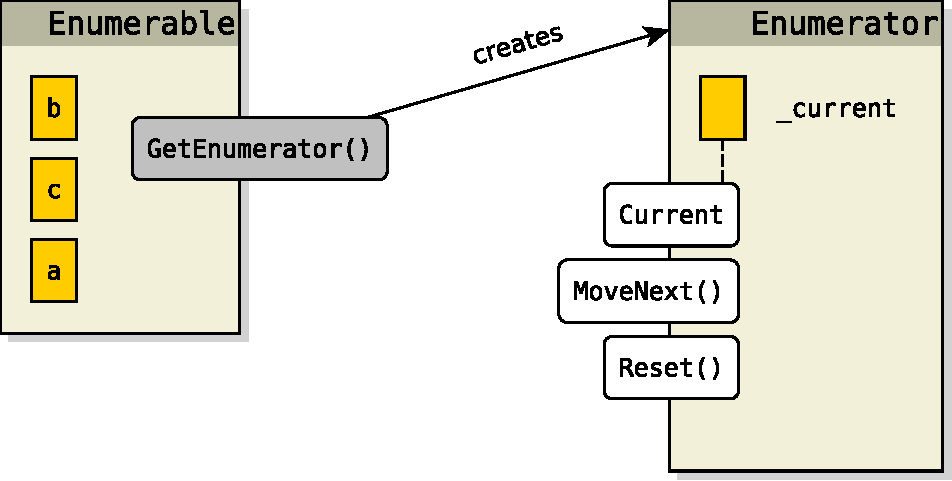
\includegraphics[width=.8\linewidth]{img/enumeration-1.pdf}
  
  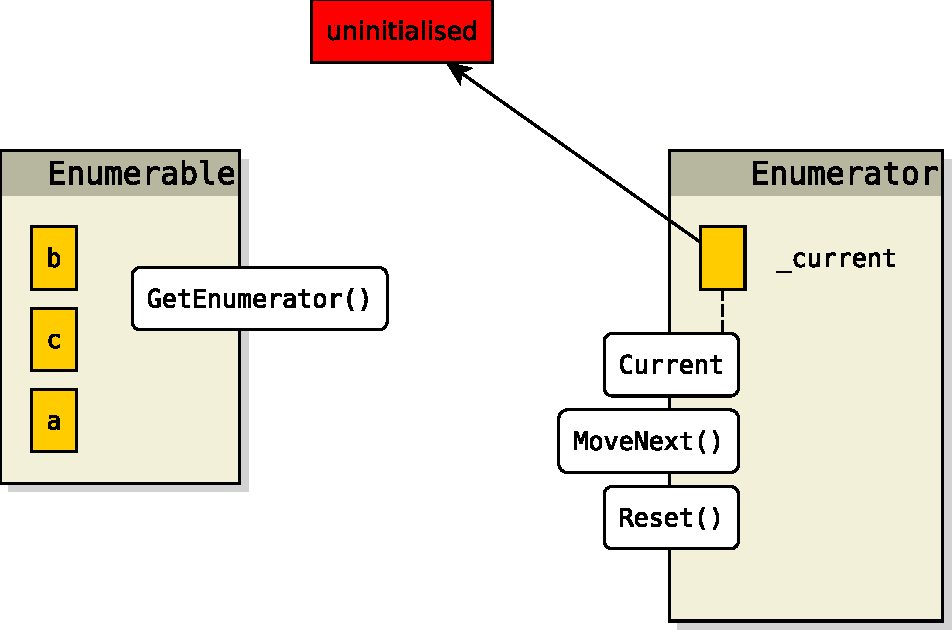
\includegraphics[width=.8\linewidth]{img/enumeration-2.pdf}
  
  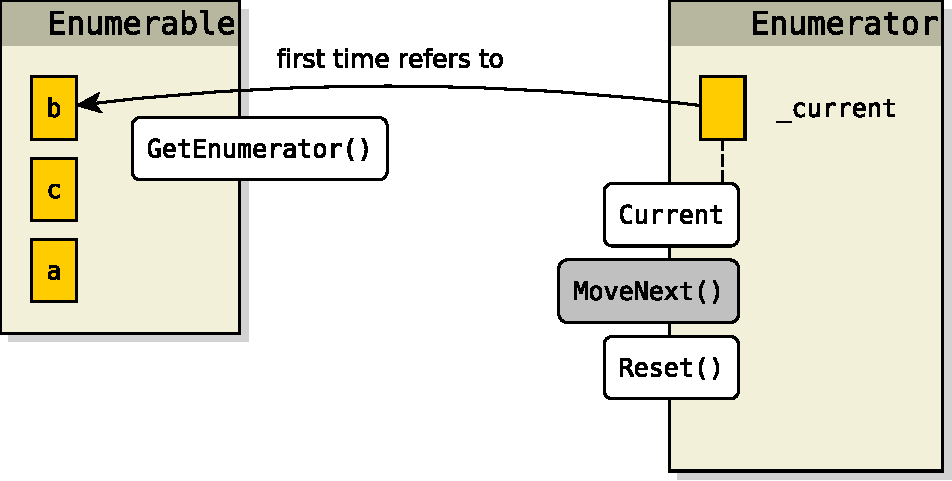
\includegraphics[width=.8\linewidth]{img/enumeration-3.pdf}
  
  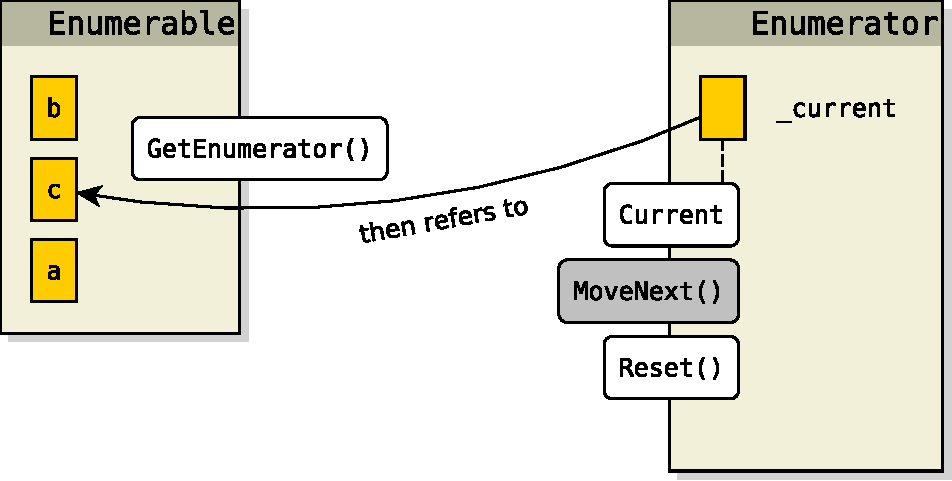
\includegraphics[width=.8\linewidth]{img/enumeration-4.pdf}
  
  \includegraphics[width=.8\linewidth]{img/enumeration-5.pdf}
  
  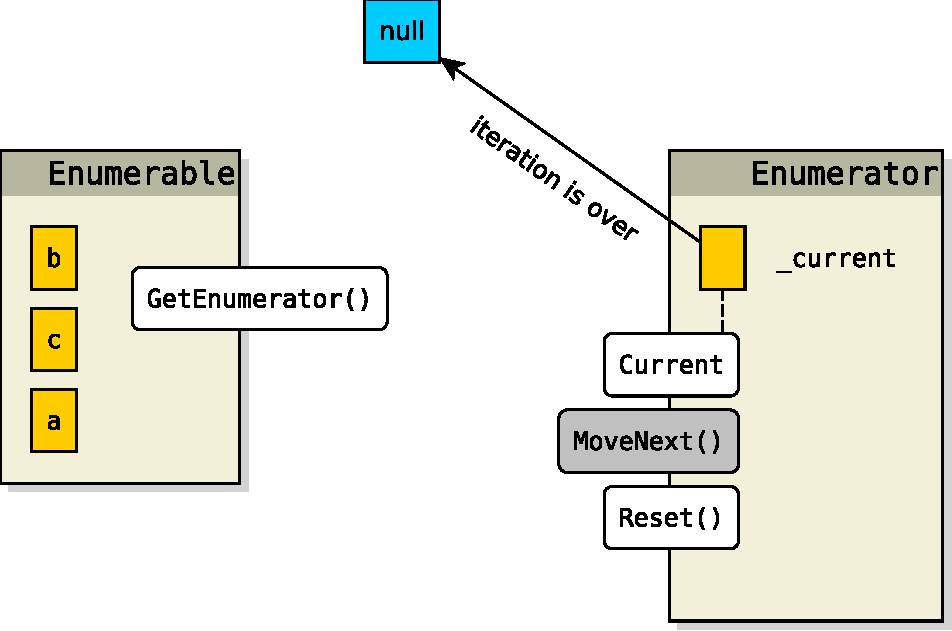
\includegraphics[width=.8\linewidth]{img/enumeration-6.pdf}

  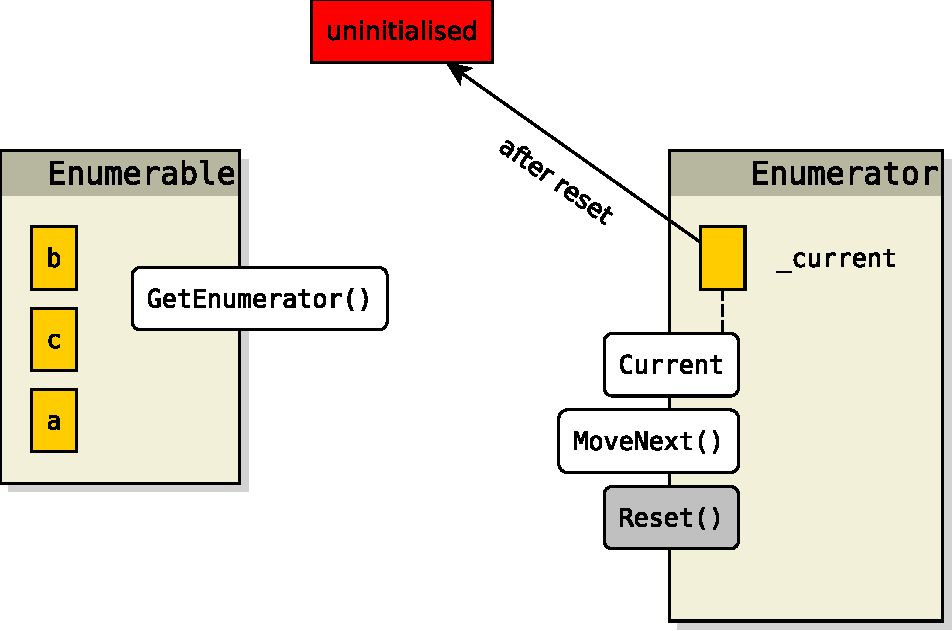
\includegraphics[width=.8\linewidth]{img/enumeration-7.pdf}

  \tcodeview{3}{17}{24}{\tiny}{\codepath{ForEach/Program.cs}}{Iterating overn an enumerable using an enumerator}

\end{frame}

\begin{frame}{Enumerables and Enumerators}
  \begin{exampleblock}{Remarks}
    \begin{itemize}
      \item They allow clients to iterate over any container of data
      %
      \begin{itemize}
        \item without needing to know \alert{how} data is enumerated
      \end{itemize}
  
      \item Enumerators, in particular, just need to memorise one item at a time
      %
      \begin{itemize}
        \item[$\rightarrow$] they can iterate over \alert{possibly infinite} amounts of data
      \end{itemize}

      \item They are the mechanism behind the \alert{\texttt{for-each}} construct!
      %
      \begin{itemize}
        \item each \texttt{for-each} execution creates a new enumerator behind the scenes
        \item this is why all objects which can create an enumerator can be iterated via \texttt{for-each}
        \item this is why \texttt{for-each} can be executed on all enumerables
      \end{itemize}
    \end{itemize}
  \end{exampleblock}
\end{frame}

\subsection{Indexers}

\begin{frame}[allowframebreaks]{Indexers}

  \begin{block}{Indexers in a Nutshell}
    \begin{itemize}
      \item Indexers are \alert{syntactic sugar} for \alert{accessing} collections' item with \alert{array-like syntax}
      \item They are used extensively in \dotnet collection types
      \item You must know how to \alert{use} them, to \alert{use} collections
      \item You must know how to \alert{write} them, to \alert{create} custom collections
    \end{itemize}
  \end{block}

  \begin{block}{Indexers' Syntax}
    \begin{itemize}
      \item Indexers are another possible sort of class \alert{members}
      \item Indexers are essentially \alert{properties} with \alert{arguments}
      %
      \begin{itemize}
        \item while name is \alert{\texttt{this}}
        \item which are used via the \alert{sequare brackets} syntax
      \end{itemize}
    \end{itemize}
  \end{block}
  
  \tcodeview{1}{11}{25}{\tiny}{\codepath{Indexers/Program.cs}}{Definition of an Indexer}

  \tcodeview{2}{29}{40}{\tiny}{\codepath{Indexers/Program.cs}}{Usage of an Indexer}

\end{frame}

\subsection{Collection Items}

\begin{frame}[allowframebreaks]{About Collection Items}
  \begin{block}{Recall the basis of OOP in \dotnet}
    \begin{itemize}
      \item All objects are instances of the \texttt{Objects} class
      \item All instances inherit from \texttt{Object} (at least) the following methods:
      %
      \begin{description}
        \item[\texttt{bool Equals(object)}] which returns true if the current object is equal to the provided one
        \item[\texttt{int GetHashCode()}] which returns the same integer for all objects which are equal 
        \item[\texttt{string ToString()}] which returns an intelligible representation of the object as a string
      \end{description}
    \end{itemize}
  \end{block}

  \tcodeview{1}{5}{16}{\tiny}{\codepath{Items/Program.cs}}{The \texttt{Object} class}

  \begin{block}{Semantics of \texttt{Equals} and \texttt{HashCode}}
    \begin{itemize}
      \item Overriding \texttt{Equals} in a type means reifying a particular equality notion for that type
      \item Not overriding \texttt{Equals} in a type means that \alert{equality $\equiv$ identity}
      \item A valid equality notion must be:
      %
      \begin{itemize}\scriptsize
        \item \alert{reflexive}, i.e. \texttt{x.Equals(x)} for all possible \texttt{x} 
        \item \alert{symmetric}, i.e. \texttt{x.Equals(y) == y.Equals(x)} for all possible \texttt{x}, \texttt{y} 
        \item \alert{transitive}, i.e. if \texttt{x.Equals(y) == true} and \texttt{y.Equals(z) == true}, then \texttt{x.Equals(z) == true}  for all possible \texttt{x}, \texttt{y}, and \texttt{z}
        \item \alert{deterministic}, i.e. \texttt{x.Equals(y)} always provides the same result for the same \texttt{x}, \texttt{y} 
        \item furthermore, \texttt{x.Equals(null) == false} for all possible \texttt{x} 
      \end{itemize}

      \item Similarly, an implementation of \texttt{HashCode} is valid only if it is:
      %
      \begin{itemize}
        \item \alert{coherent} w.r.t. the equality notion
        \item[ie] \texttt{x.GetHashCode() == y.GetHashCode()} for all \texttt{x}, and \texttt{y}  such that \texttt{x.Equals(y) == true}
      \end{itemize}
    \end{itemize}
  \end{block}

  \begin{alertblock}{Requirements on collection items}
    All classes whose instances need to be used as collection items:
    %
    \begin{itemize}
      \item \alert{must} provide a valid implementation for both \texttt{Equals} and \texttt{GetHashCode}
      %
      \begin{itemize}
        \item[!] otherwise collections \alert{won't work} consistently with those classes
      \end{itemize}
      
      % \begin{itemize}
      %   \item 
      % \end{itemize}
      \item \alert{should} provide a valid implementation for \texttt{ToString}
      %
      \begin{itemize}
        \item this is not mandatory but it is useful for debugging and presentation
      \end{itemize}

      \item IDEs usually provide some means to \alert{automatically generate} valid implementations for these methods
    \end{itemize}

  \end{alertblock}

  \tcodeview{1}{5}{17}{\tiny}{\codepath{Items/Wrong/Person.cs}}{Wrong \texttt{Person} class}
  \codeview{3}{23}{27}{\tiny}{\codepath{Items/Wrong/Person.cs}}

  \tcodeview{1}{5}{22}{\tiny}{\codepath{Items/Correct/Person.cs}}{Correct \texttt{Person} class}
  \codeview{3}{28}{32}{\tiny}{\codepath{Items/Correct/Person.cs}}

  \begin{exampleblock}{Best Practices}
    \begin{itemize}
      \item Classes not needing to implement \texttt{Equals} and \texttt{GetHashCode} are rare
      \item Meaningful implementations of \texttt{ToString} are always very useful
      \item Suggestion:
      %
      \begin{itemize}
        \item always implement \texttt{Equals}, \texttt{GetHashCode}, and \texttt{ToString}, by default
        \item remove them when their lack is an explict requirement
      \end{itemize}
    \end{itemize}
  \end{exampleblock}

  \begin{exampleblock}{Rule of thumbs for implmenting \texttt{Equals} and \texttt{GetHashCode}}
    \begin{itemize}
      \item Implement \texttt{Equals} first
      %
      \begin{enumerate}
        \item perform null-check first, return false in case of null object
        \item perform reference-equality short circuiting, return true if successful
        \item check if type of the two object is the same, return false if not
        \item cast the object to the current type
        \item compare the public properties of the two objects
        %
        \begin{itemize}
          \item ask yourself ``which properties make two instances equal''?
        \end{itemize}
      \end{enumerate}

      \item Implement \texttt{GetHashCode} next
      %
      \begin{enumerate}
        \item combine the same properties compared in \texttt{Equals}, no more, no less
        \item use the \texttt{HashCode.Combine} static method
      \end{enumerate}
    \end{itemize}
  \end{exampleblock}
\end{frame}

\subsection{Using Collections}

\begin{frame}[allowframebreaks]{The \texttt{ICollection<T>} Interface}

  \tcodeview{1}{6}{28}{\tiny}{\codepath{Collections/ICollection.cs}}{The \texttt{System.Collections.Generic.ICollection<T>} Interface}

  \begin{block}{Creation}
    \begin{itemize}
      \item By instantiating any class which \alert{directly or indirectly} implements \texttt{ICollection<T>}
      %
      \begin{itemize}
        \item[eg] \texttt{System.Collections.ObjectModel.\alert{Collection<T>}}
      \end{itemize}
      
      \item \alert{Declare} the variable using the \alert{interface}, \alert{initialise} it using a \alert{class}
      
      \item Use the following syntax to provide \alert{items} on the fly:
      %
      \begin{center}\ttfamily
        new \cscat{Collection Class}() \{ \cscat{Item$_1$}, \ldots, \cscat{Item$_N$} \}
      \end{center}
      
      \begin{itemize}
        \item where all \texttt{\cscat{Item$_i$}} are expressions returning instances of \alert{\texttt{T}}
      \end{itemize}
    \end{itemize}
  \end{block}

  \begin{block}{Usage}
    \begin{itemize}
      \item The metods of \texttt{ICollection<T>} support all basic operations
      %
      \begin{itemize}
        \item except directly reading a particular item
      \end{itemize}
      \item By default, they support a \alert{mutable} operation approach
      \item Converting a collection into string \alert{does not shows its items}!
    \end{itemize}
  \end{block}

  \framebreak

  \tcodeview{3}{36}{61}{\tiny}{\codepath{CollectionUsages/Program.cs}}{Creating/Usage example for the \texttt{Collection} class}
  
\end{frame}

\subsection{Using Lists}

\begin{frame}[allowframebreaks]{The \texttt{IList<T>} Interface}

  \tcodeview{1}{6}{23}{\tiny}{\codepath{Collections/IList.cs}}{The \texttt{System.Collections.Generic.IList<T>} Interface}

  \begin{block}{Creation}
    \begin{itemize}
      \item By instantiating any class which \alert{directly or indirectly} implements \texttt{IList<T>}
      %
      \begin{itemize}
        \item[eg] \texttt{System.Collections.Generic.\alert{List<T>}}
      \end{itemize}
      
      \item \alert{Declare} the variable using the \alert{interface}, \alert{initialise} it using a \alert{class}
      
      \item Use the followin syntax to provide \alert{items} on the fly:
      %
      \begin{center}\ttfamily
        new \cscat{List Class}() \{ \cscat{Item$_1$}, \ldots, \cscat{Item$_N$} \}
      \end{center}
      
      \begin{itemize}
        \item where all \texttt{\cscat{Item$_i$}} are expressions returning instances of \alert{\texttt{T}}
      \end{itemize}
    \end{itemize}
  \end{block}

  \framebreak

  \begin{block}{Usage}
    \begin{itemize}
      \item The metods of \texttt{IList<T>} support all basic operations
      %
      \begin{itemize}
        \item including directly accessing a particular item, by \alert{index}
        \item including discovering the \alert{indexing} of an item
      \end{itemize}
      \item By default, they support a \alert{mutable} operation approach
      \item Converting a list into string \alert{does not show its items}!
    \end{itemize}
  \end{block}

  \framebreak

  \tcodeview{3}{66}{91}{\tiny}{\codepath{CollectionUsages/Program.cs}}{Creating/Usage example for the \texttt{List} class}
  
\end{frame}

\subsection{Using Sets}

\begin{frame}[allowframebreaks]{The \texttt{ISet<T>} Interface}

  \tcodeview{1}{6}{48}{\tiny}{\codepath{Collections/ISet.cs}}{The \texttt{System.Collections.Generic.ISet<T>} Interface}

  \begin{block}{Creation}
    \begin{itemize}
      \item By instantiating any class which \alert{directly or indirectly} implements \texttt{ISet<T>}
      %
      \begin{itemize}
        \item[eg] \texttt{System.Collections.Generic.\alert{HashSet<T>}}
        \item[eg] \texttt{System.Collections.Generic.\alert{SortedSet<T>}}
        %
        \begin{itemize}
          \item where items are stored in \alert{orderly} fashion
        \end{itemize} 
      \end{itemize}
      
      \item \alert{Declare} the variable using the \alert{interface}, \alert{initialise} it using a \alert{class}
      
      \item Use the following syntax to provide \alert{items} on the fly:
      %
      \begin{center}\ttfamily
        new \cscat{Set Class}() \{ \cscat{Item$_1$}, \ldots, \cscat{Item$_N$} \}
      \end{center}
      
      \begin{itemize}
        \item where all \texttt{\cscat{Item$_i$}} are expressions returning instances of \alert{\texttt{T}}
      \end{itemize}
    \end{itemize}
  \end{block}

  \framebreak

  \begin{block}{Usage}
    \begin{itemize}
      \item The metods of \texttt{ISet<T>} support all basic operations
      %
      \begin{itemize}
        \item plus set-related algebraic methods such as unition, intersection, super/sub-set testing, etc.
      \end{itemize}
      \item By default, they support a \alert{mutable} operation approach
      \item Converting a set into string \alert{does not show its items}!
    \end{itemize}
  \end{block}

  \framebreak

  \tcodeview{3}{96}{119}{\tiny}{\codepath{CollectionUsages/Program.cs}}{Creating/Usage example for the \texttt{HashSet} class}
  %
  \begin{itemize}
    \item consider retrying the same test with the \texttt{SortedSet<T>} class
  \end{itemize}

\end{frame}

\subsection{Using Dictionaries}

\begin{frame}[allowframebreaks]{The \texttt{IDictionary<K, V>} Interface}

  \tcodeview{1}{6}{29}{\tiny}{\codepath{Collections/IDictionary.cs}}{The \texttt{System.Collections.Generic.IDictionary<K, V>} Interface}

  \begin{block}{Creation}
    \begin{itemize}
      \item By instantiating any class which \alert{directly or indirectly} implements \texttt{IDictionary<K, V>}
      %
      \begin{itemize}
        \item[eg] \texttt{System.Collections.Generic.\alert{Dictionary<K, V>}}
        \item[eg] \texttt{System.Collections.Generic.\alert{SortedDictionary<K, V>}}
        %
        \begin{itemize}
          \item where items are stored in \alert{orderly} fashion (by keys)
        \end{itemize} 
      \end{itemize}
      
      \item \alert{Declare} the variable using the \alert{interface}, \alert{initialise} it using a \alert{class}
      
      \item Use the following syntax to provide \alert{items} on the fly:
      %
      \begin{center}\ttfamily\small
        new \cscat{Dict. Class}() \{ \kva{Key$_1$}{Val$_1$}, \ldots, \kva{Key$_N$}{Val$_N$} \}
      \end{center}
      %
      or
      %
      \begin{center}\ttfamily\small
        new \cscat{Dict. Class}() \{ \kvb{Key$_1$}{Val$_1$}, \ldots, \kvb{Key$_N$}{Val$_N$} \}
      \end{center}
      
      \begin{itemize}
        \item where all \texttt{\cscat{Key$_i$}} are expressions returning instances of \alert{\texttt{K}}
        \item where all \texttt{\cscat{Val$_i$}} are expressions returning instances of \alert{\texttt{V}}
      \end{itemize}
    \end{itemize}
  \end{block}

  \framebreak

  \begin{block}{Usage}
    \begin{itemize}
      \item The metods of \texttt{IDictionary<K, V>} support all common collections operations\ldots
      %
      \begin{itemize}
        \item \ldots on key-value pairs
        \item plus some key-specific operations
      \end{itemize}
      \item By default, they support a \alert{mutable} operation approach
      \item Converting a map into string \alert{does not show its items}!
    \end{itemize}
  \end{block}

  \framebreak

  \tcodeview{3}{124}{163}{\tiny}{\codepath{CollectionUsages/Program.cs}}{Creating/Usage example for the \texttt{Dictionary} class}
  %
  \begin{itemize}
    \item consider retrying the same test with the \texttt{SortedDictionary<K, V>} class
  \end{itemize}

\end{frame}

\subsection{Using Tuples}

\begin{frame}[allowframebreaks]{The \texttt{Tuple<T1, T2, ...>} Classes}

  \tcodeview{1}{3}{23}{\tiny}{\codepath{Collections/Tuple.cs}}{The \texttt{System.Tuple<T1, T2, ...>} Class}

  \begin{block}{Creation}
    \begin{itemize}
      \item Using the static factory methods in \alert{\texttt{System.Tuple}}
      %
      \begin{itemize}
        \item[eg] \texttt{Create\alert{<T1, T2>}}
        \item[eg] \texttt{Create\alert{<T1, T2, T3>}}
        \item[\vdots]
        \item[eg] \texttt{Create\alert{<T1, T2, T3, T4, T5, T6, T7, T8>}}
      \end{itemize}
            
      \item No interfaces involved in this case!
      
      \item Notice that there exist 8+1 classes named \texttt{Tuple} in \texttt{System}
      %
      \begin{itemize}
        \item one having 1 generic variable, one having 2 generic variables, \ldots
        \item one containing static factories
      \end{itemize}
      
    \end{itemize}
  \end{block}

  \framebreak

  \begin{block}{Usage}
    \begin{itemize}
      \item Tuples can be used to carry a number of typed data together, without having to create an ad-hoc class
      \item They can only be created, compared, converted into string, and carried around
      \item Specific items can be retrived via ad-hoc properties, via the syntax
      %
      \begin{center}\ttfamily
        \cscat{Tuple}.Item\cscat{N}
      \end{center}
      %
      \begin{itemize}
        \item where \texttt{\cscat{Tuple}} is an expression returning a tuple 
        \item and \texttt{\cscat{N}} is an integer between 1 and 8
      \end{itemize}
    \end{itemize}
  \end{block}

  \framebreak

  \tcodeview{3}{168}{185}{\tiny}{\codepath{CollectionUsages/Program.cs}}{Creating/Usage example for the \texttt{Dictionary} class}

\end{frame}

\subsection{Notable Remarks}

\begin{frame}[allowframebreaks]{Notable Remarks about \dotnet Collections}

  Consider the following statements as \alert{default}, unless the documentation of a particular collection states otherwise:
  %
  \bigskip
  %
  \begin{itemize}
    \item The method \texttt{ToString()} of any collection returns a string which \alert{does not} represent the collection's items
    %
    \begin{itemize}
      \item to quickly represent the collection items as string, you may write:
      %
      \begin{center}
        \lstinline[basicstyle=\normalsize\ttfamily]{string.Join(", ", collection)}
      \end{center}
    \end{itemize}

    \bigskip

    \item The method \texttt{Equals(object)} of any collection only checks for \alert{identity}
    %
    \begin{itemize}
      \item items are not taken into account for comparisons among collections
      \item to quickly compare two collections of the same sort you may exploit
      %
      \begin{center}
        \lstinline[basicstyle=\footnotesize\ttfamily]{System.Linq.Enumerable.SequenceEqual(collection1, collection2)}
      \end{center}
      %
      \begin{itemize}
        \item which checks if two enumerables contain \alert{equal items in the same order}
      \end{itemize}
    \end{itemize}

    \bigskip

    \item The method \texttt{GetHashCode()} of any collection does not take items into account
    %
    \begin{itemize}
      \item you \alert{cannot} simply use \alert{sets as keys} for dictionaries, nor create \alert{sets of sets}
    \end{itemize}

    \bigskip

    \item Collection \alert{classes} commonly expose a public constructor which accept another \alert{enumerable} as input
    %
    \begin{itemize}
      \item use these constructors to create an instance of a collection containing the items of another collection
      %
      \begin{itemize}
        \item[eg] a \alert{copy} of the former collection
      \end{itemize}
    \end{itemize}
  \end{itemize}
  
\end{frame}

\section{Comparers}

\begin{frame}[allowframebreaks]{Orderings and Comparers}
  \begin{alertblock}{Question}\centering
    How can classes \texttt{SortedSet} and \texttt{SortedDictionary} \alert{sort} their items?
  \end{alertblock}

  \begin{block}{Sort and Ordering}\centering
    \begin{itemize}
      \item Sorting means enumerating a number of items according to a given \alert{ordering criterion}
      \item An ordering criterion is a way to say:
      %
      \begin{itemize}
        \item if an item is \alert{greater} than another
        %
        \begin{itemize}
          \item i.e. if it comes \alert{after} the other in the enumeration
        \end{itemize}
        \item if an item is \alert{lower} than another
        %
        \begin{itemize}
          \item i.e. if it comes \alert{before} the other in the enumeration
        \end{itemize}
      \end{itemize}
    \end{itemize}
  \end{block}

  \begin{exampleblock}{Comparers}
    \begin{center}\itshape
      Comparers are the way \alert{ordering criteria} are reified into code, in \dotnet
    \end{center}
  \end{exampleblock}

  \tcodeview{1}{3}{11}{\tiny}{\codepath{Collections/IComparer.cs}}{The \texttt{System.Collections.Generic.IComparer<T>} Class}

  \bigskip

  Remarks:
  %
  \begin{itemize}
    \item by creating a comparer for some \texttt{T}, you may allow \dotnet built-in classes to sort items
    \item classes suc as \texttt{SortedSet} and \texttt{SortedDictionary} usually expose a constructor accepting a comparer for their items
    %
    \begin{itemize}
      \item in case this is missing, they rely on a default comparer
    \end{itemize}
  \end{itemize}

\end{frame}

\begin{frame}[allowframebreaks]{Comparer Example -- \texttt{PersonComparer}}
    Consider the good, old-fashioned \texttt{Person} class:
    %
    \codeview{1}{3}{10}{\tiny}{\codepath{Comparers/Person.cs}}
    
    and the following comparer classes:
    %
    \codeview{1}{5}{9}{\tiny}{\codepath{Comparers/PersonComparer.cs}}
    %
    \begin{itemize}
      \item why do this work?
    \end{itemize}
    %   
    \framebreak
    %
    \codeview{1}{11}{15}{\tiny}{\codepath{Comparers/PersonComparer.cs}}
    %
    \begin{itemize}
      \item notice that this leverages on the default comparer for strings
    \end{itemize}
    %
    \codeview{1}{17}{31}{\tiny}{\codepath{Comparers/PersonComparer.cs}}

    \framebreak

    suppose now you have a bunch of people to be sorted:
    %
    \codeview{3}{11}{16}{\tiny}{\codepath{Comparers/Program.cs}}
    %
    then, each comparer enables sorting them with a different criterion:
    %
    \codeview{3}{18}{25}{\tiny}{\codepath{Comparers/Program.cs}}
    %
    % \codeview{3}{21}{22}{\tiny}{\codepath{Comparers/Program.cs}}
    % %
    % \codeview{3}{24}{25}{\tiny}{\codepath{Comparers/Program.cs}}
    
\end{frame}

\frame[label=coverpage]{\titlepage}

\end{document}
